\chapter{实验}

在本章中,我们将评估视频压缩算法的性能。我们同时给了直观的例子和具体的
评估数据。我们使用标准的 PSNR 值作为指标来评估视频压缩质量。

\section{选点的评估}

首先我们将在选择最有代表性的点上对比我们的算法和 Cheng 的方法。我们使
用 \cite{learning-to-compress-images} 中使用的那个接线员的视频来进行实
验。该视频一共有 301 帧,每一帧的大小是 $240 \times 130$。

图 \ref{fig:tm-compare}a 和 \ref{fig:tm-compare}d 给出了第一帧和对应的
灰度图像。图 \ref{fig:tm-compare}b 和 \ref{fig:tm-compare}e 分别给出
了Cheng 的主动学习算法和我们的主动学习算法说选出来的像素点。两种算法各
选了 500 个点,可以看到,相比于 Cheng 的算法,我们的方法在颜色改变的边
界处选择了更多的点,从我们的算法选出来的点的分布可以大致看出一个人脸的
轮廓。图 \ref{fig:tm-compare}c 和 \ref{fig:tm-compare}f 给出了 Cheng
和我们的方法着色(和解压缩)的结果。可以看到,我们的方法给出了视觉上更
好的结果。对于第一帧,Cheng 的方法得出的 PSNR 是 $35.38$,我们的方法是
$38.99$,比 Cheng 的方法明显要高。

\section{视频压缩质量的评估}

这个实验的目的是从视频压缩的质量上来比较我们的方法和 Cheng 的方法。通过
固定总的选点数目的办法,我们将压缩比设定为一个固定值,有此通过比较
PSNR 值的办法来衡量视频压缩的质量。

在视频压缩的过程中训练的模型的个数依赖于 $\Delta_{PSNR}$ 和着色的质量。
在这个实验中,Cheng 的方法一共训练了 9 个模型,而我们的 SFM 和 MFM 方
法分布训练了 9 个和 3 个模型。要让各个方法选点的总数完全一样几乎是不可
能的事,对于 Cheng 的方法,每次重新训练模型的时候都会选择 500 个点,因
此一共选择了 4500 个点,我们的 SFM 也是一样,因此一共也是选择了 4500
个点,而对于 MFM 来说,我们并没有将每次选点的个数设定为一个固定值,而
是选择足够多的点,使得其 PSNR 值不会低于 SFM ,在这个实验中,MFM 所选
点的总数是 3900 。

我们使用 {\em MPlayer's Movie Encoder} 来将原始视频编码为 MPEG-4 的格
式,占用的大小为 756,586 字节。然后我们用同样的编码方式将该视频编码为灰
度格式,得到的结果占用 250,288 字节。该灰度视频会在解码的时候用到。为
了恢复灰度视频,除了灰度视频之外,我们还需要存储选出来的点的空间信息和
颜色值。因此,我们需要额外的 4 个字节来存储每一个选定的点的信息(2 个
字节来存储颜色信息,2 个字节存储位置信息)。因此,Cheng 的方法和 SFM
都需要额外 18,000 字节的存储空间,而 MFM 只需要 15,600 字节。

在图 \ref{fig:telemarket}a 中,我们给出了原始视频的 48 帧,黄颜色的标记
标识了我们的算法训练模型的帧,而红色的标记则标识了 Cheng 的算法训练模型
的帧。可以看到,在第二个红色的标记的地方(第 6 行,第 2 列),该帧和前
面的帧的差别并不是特别大,然而 Cheng 的方法却在这里选择重新训练一个模
型,这是不必要的。相比起来,对于每个黄颜色的标记,我们都可以看到对应的
帧和其之前的帧是有比较大的差别的,我们的算法只在这些帧上训练新的模型。
图 \ref{fig:telemarket}b 给出了我们的方法所恢复出来的视频的对应帧。

为了比较不同算法的视频压缩的质量,我们在图 \ref{fig:psnr-more}a 中画出
了每一帧的 PSNR 值,其中横坐标是视频的帧,而纵坐标是对应的帧所恢复出来
的结果的 PSNR 值。我们还在训练模型的帧所在的地方绘制了实心圆,并且圆的
大小正比于该模型选点的数目。可以看到,在总的选点数差不多相等(亦即压缩
比相等)的情况下,我们的 SFM 和 MFM 给出的 PSNR 值比 Cheng 的方法要高许
多。具体来说,Cheng 的方法、我们的 SFM 还有 MFM 所得到的 {\em overall}
PSNR \cite{wavelet-based-rate-scalable-video-compression}值分别
是 $34.8$,$38.0$和$38.4$。

表格 \ref{tab:more-example} 给出了一些其他的视频压缩的结果\footnote{所
  有的视频都可以在 \url{http://trace.eas.asu.edu/yuv/index.html} 下载
  到。},对应的 PSNR 图也可以在图 \ref{fig:psnr-more} 中找到。在这里我
们同时还比较了标准的 MPEG-4 视频压缩的结果,我们将原始视频用标准的
MPEG-4 编码器压缩到一个差不多的压缩率,然后计算结果的 PSNR 。从表中可
以看到,在压缩比差不多的情况下,我们的方法可以得到的 PSNR 比 Cheng 的
方法要高许多,并且有时候比标准的 MPEG-4 还要好。

\begin{figure*}[t]
  \centering
  \subfigure[telemarket]{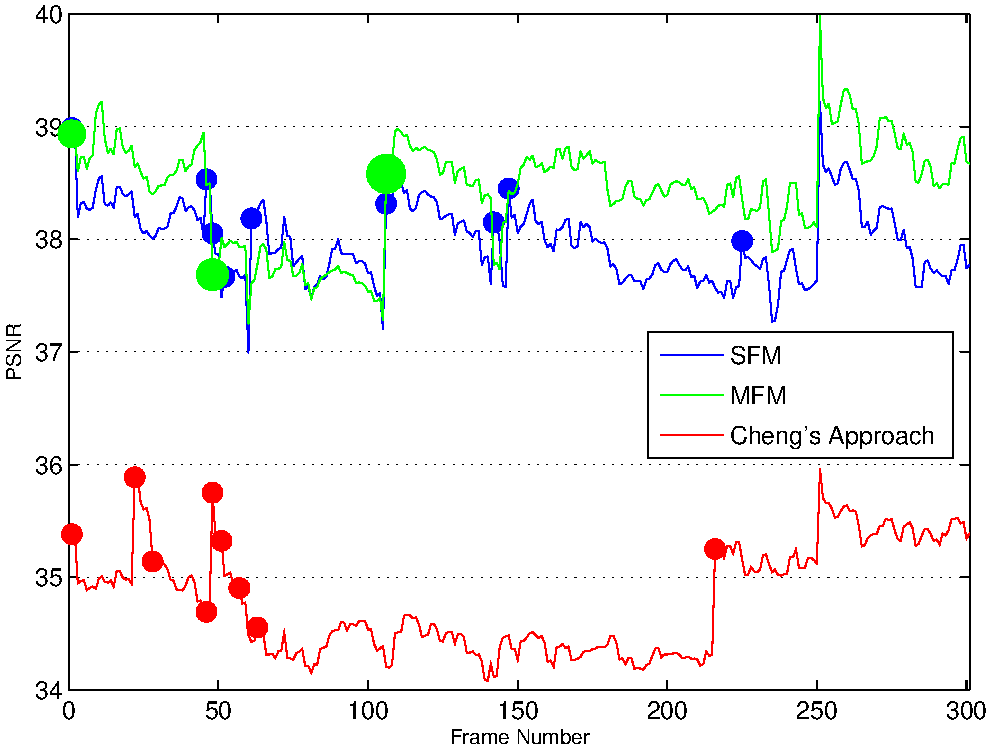
\includegraphics[width=.4\linewidth]{images/telemarket}}
  \subfigure[claire]{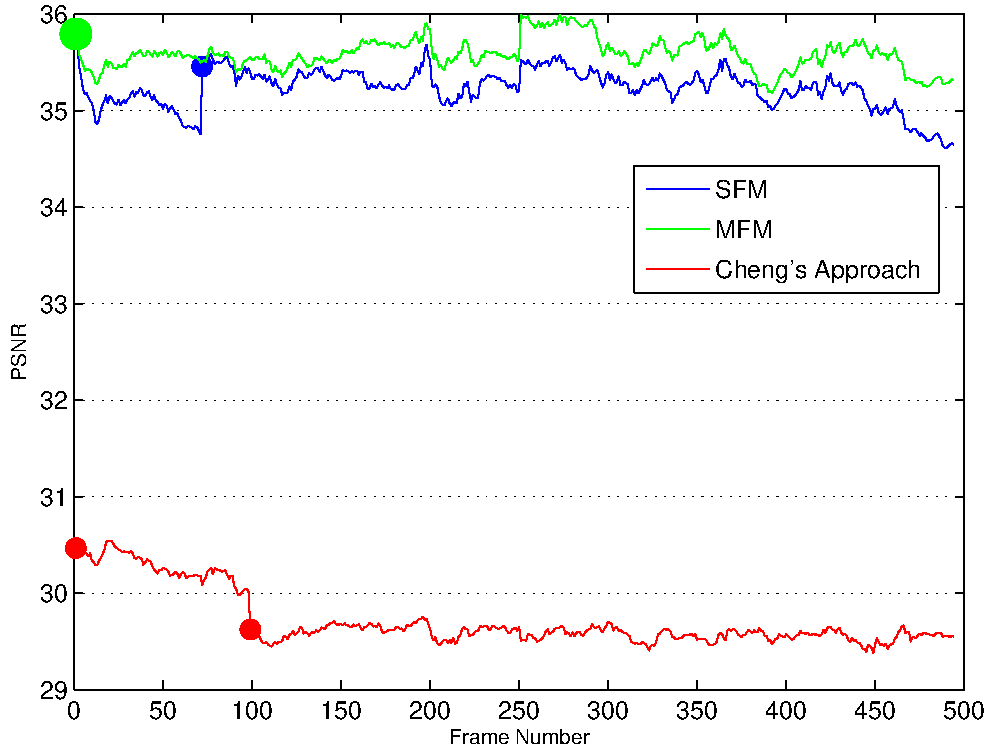
\includegraphics[width=.4\linewidth]{images/claire}}
  \subfigure[miss-america]{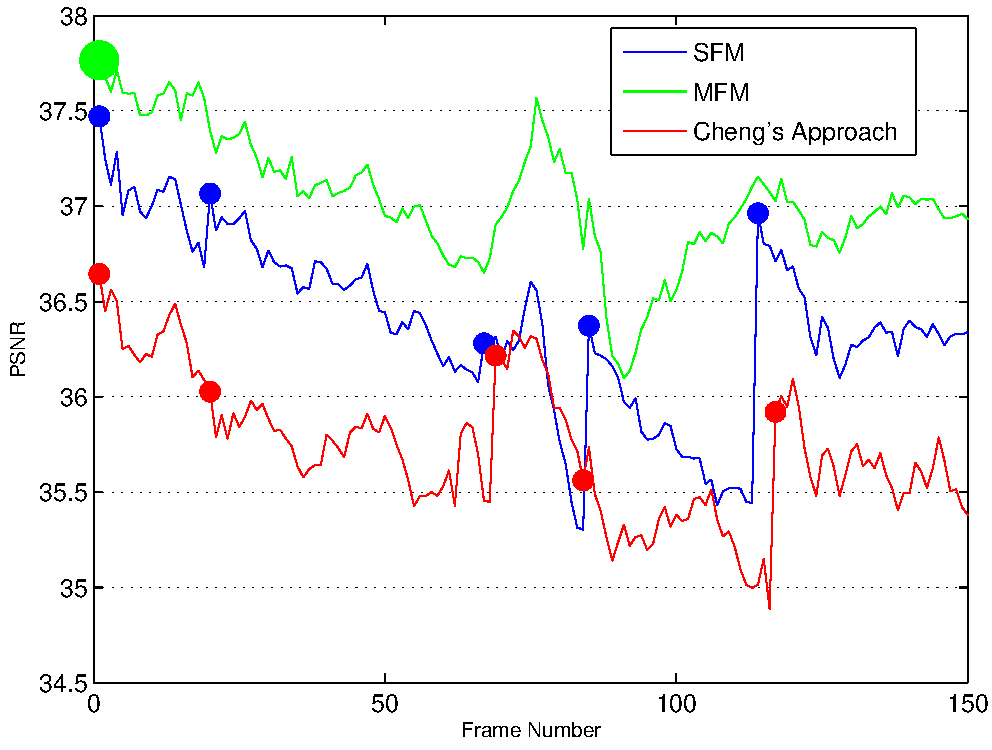
\includegraphics[width=.4\linewidth]{images/miss-america}}
  \subfigure[akiyo]{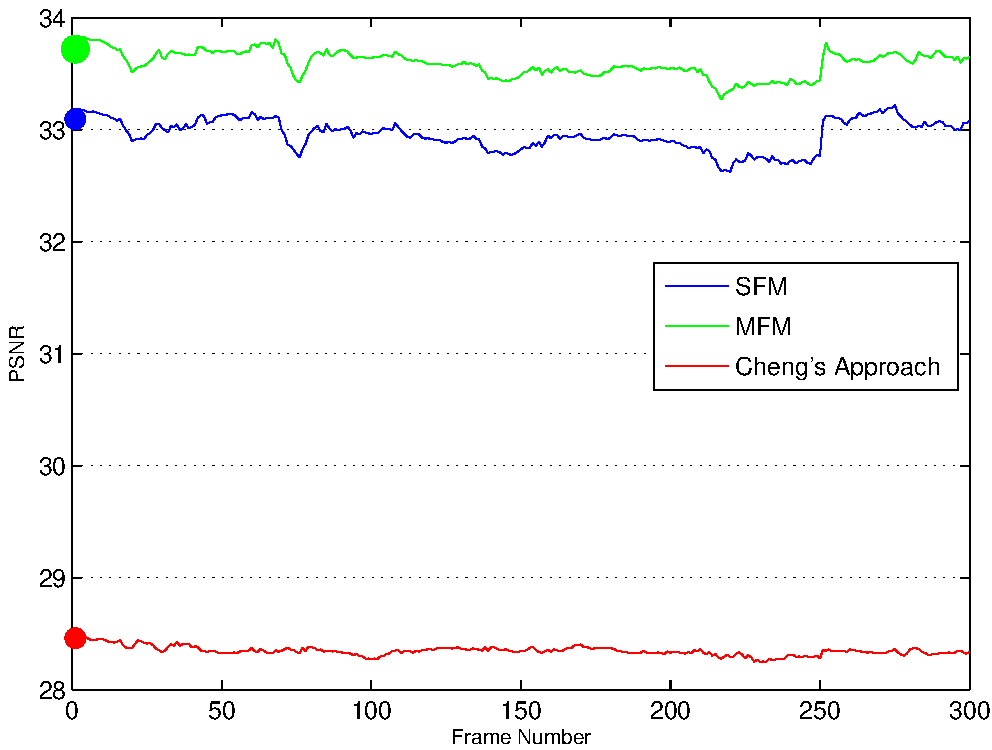
\includegraphics[width=.4\linewidth]{images/akiyo}}
  \subfigure[suzie]{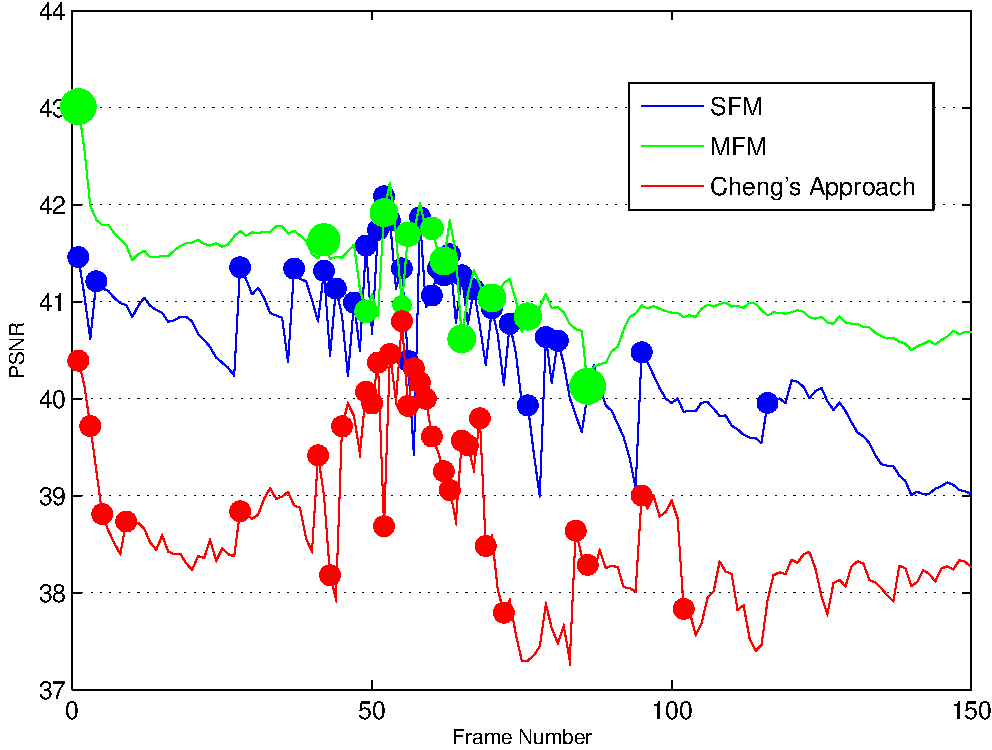
\includegraphics[width=.4\linewidth]{images/suzie}}
  \subfigure[mother-daughter]{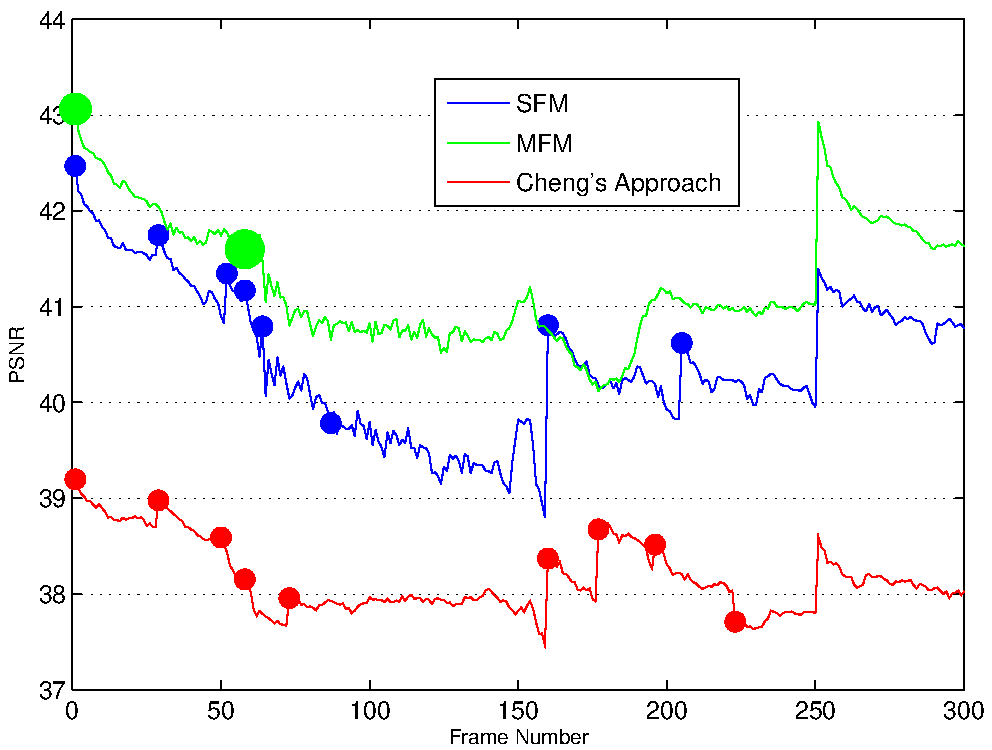
\includegraphics[width=.4\linewidth]{images/mother-daughter}}
  \caption{PSNR 图。我们的方法比 Cheng 的方法得到的 PSNR 要高许多。}
\label{fig:psnr-more}
\end{figure*}

